\section{Modos de juego}

\subsection{DeathMatch}
\emph{DeathMatch} se ubica en un pequeño mapa simétrico que enfrenta a los dos equipos en un continuo enfrentamiento, donde el objetivo es matar a los oponentes 5 veces.

\begin{figure}[H]
	\centering
	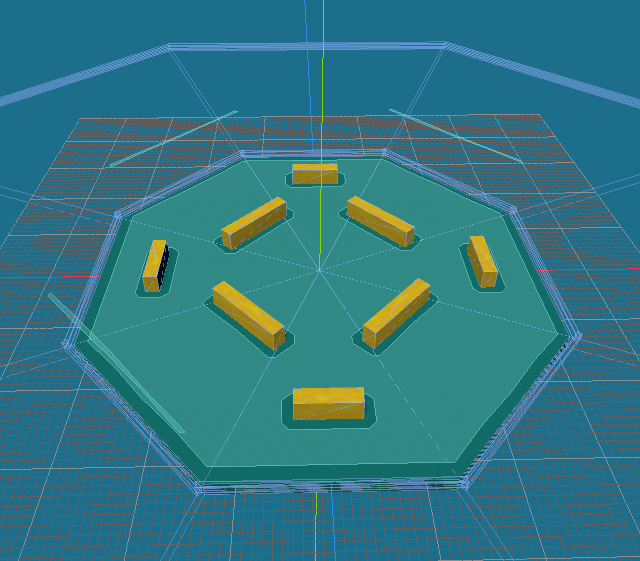
\includegraphics[width=0.5\linewidth]{figures/DeathMatchStage.png}
	% \caption{Escenario para el modo de juego DeathMatch.}
	\label{fig:DeathMatchStage}
\end{figure}

\vspace{\baselineskip}

\subsection{Captura}
Mapa grande donde los jugadores deben defender la zona del hada (la cual se va desplazando continuamente) el mayor tiempo posible. Los equipos reciben puntos por cada jugador que esté dentro de la zona en cada instante de tiempo. Una vez que han pasado 5 minutos, el equipo con más puntos gana.

\vspace{\baselineskip}

El mapa tiene tres tipos de zonas: la fortaleza central, las fortalezas de las esquinas y las zonas \emph{de paso}. Las fortalezas de las esquinas son fáciles de defender, al tener solo dos aperturas. La fortaleza central es más difícil de defender, al tener cuatro aperturas. Las zonas \emph{de paso} son zonas abiertas por las que se mueve el hada de una fortaleza a otra.

\begin{figure}[H]
	\centering
	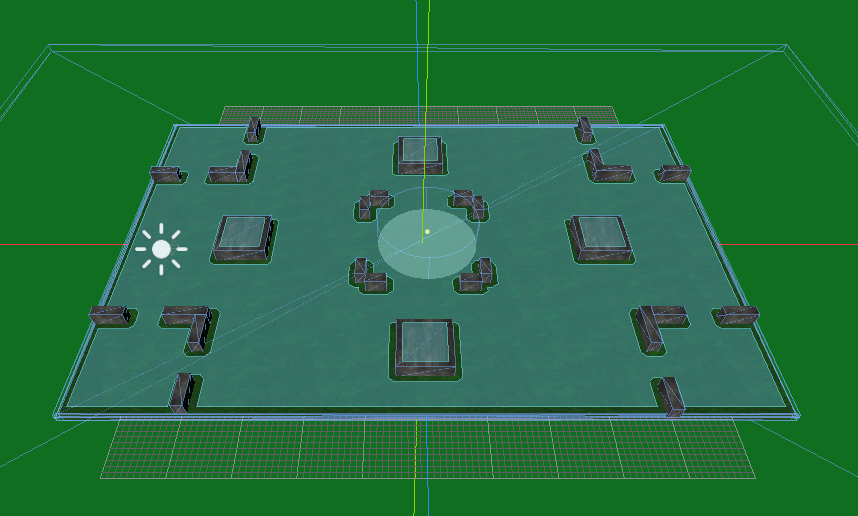
\includegraphics[width=0.7\linewidth]{figures/CaptureStage.png}
	% \caption{Escenario para el modo de juego Captura.}
	\label{fig:CaptureStage}
\end{figure}